\section{Motors}\label{motors}

Let $G$ be a graph. Suppose we wish to study the periodic behavior of games on
$G$, focusing on a particular subgraph $H \subseteq G$. Consider
\begin{equation*}
  X = \set{v \in \V \setminus \V[H]}{\N{v} \cap \V[H] \neq \emptyset},
\end{equation*}
the set of vertices ``just outside'' of $H$. Knowing the initial chip
configuration on $\V[H] \cup X$ is in general not enough to determine all
subsequent configurations because vertices in $X$ may have interactions with
vertices outside of $\V[H] \cup X$. However, we do know that every vertex
assumes a pattern of firing and waiting that repeats periodically as soon as a
game reaches a periodic position. Therefore, we can simulate the presence of
the rest of $G$ by having each vertex in $X$ fire with a regular pattern
regardless of the number of chips it receives.

The $\emph{firing sequence}$ of a vertex $v$ in game $\s$ is the sequence
$(\firing{v}{t})_{t \in \nats}$. A \emph{motorized parallel chip-firing game},
or simply ``motorized game'', on $G$ is a game $\s$ obeying \eqref{gameDef}
with a non-empty set of \emph{motors} $\mots \subseteq \V$. Each motor follows
a predetermined firing sequence without regard for normal chip-firing
rules. For example, a motor may have a negative number of chips. The term
``ordinary game'' refers to a game with no motors when there is ambiguity. A
motorized game is shown in Figure~\ref{motorizedTreeNoGlider}.
\begin{figure}
  \centering
  \subfloat{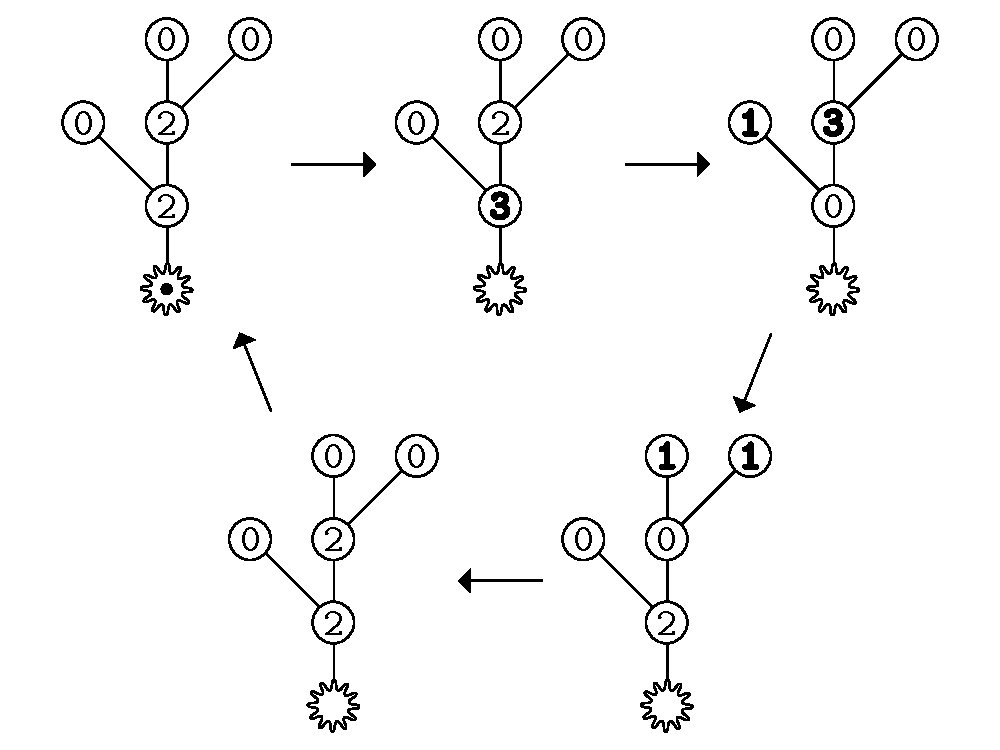
\includegraphics[width=\figWidthA]{Figures/motorizedTreeNoGlider}}
  \subfloat{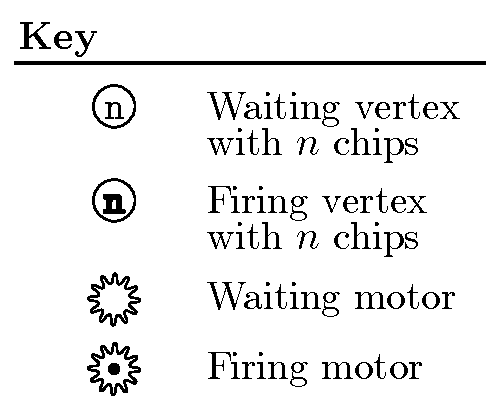
\includegraphics[width=\figWidthB]{Figures/keyShortish}}
  \caption{A motorized parallel chip-firing game. The motor has firing sequence
    $(1,0,0,0,0,1,0,0,0,0,\dots)$.}
  \label{motorizedTreeNoGlider}
\end{figure}

If a motorized game $\s$ is eventually periodic (which is the case if every
motor's firing sequence is eventually periodic), then just as in an ordinary
game, every vertex fires the same number of times each period. This is because
all neighbors of the vertex that fires the most times each period must also
fire that number of times, and therefore, by induction, so do all
vertices. (Recall that we consider in this paper only connected graphs.) This
is identical to the proof of this fact for ordinary games~\cite{jiang}.

We define
\[
  \pat{v}{f} = \set{t \in \nats}{\firing{v}{t} = f}.
\]
Call an interval $[a, b]$ with $a < b$ a \emph{max-clump} of $v \in \V$ if and
only if $[a, b] \in \pat{v}{f}$ and $\firing{v}{a-1} = \firing{v}{b+1} = 1-f$,
where $f \in \{0,1\}$. Given $v \in \V$, we can express $\nats$ as the union of
max-clumps of $v$ and times during which $v$ alternates between firing and
waiting.

The proof of Theorem~\ref{cheapLunch} follows the same structure as the proof
that ordinary games on trees have period~1 or~2~\cite{bitarGoles}. In fact, we
rely on a lemma originally introduced for that proof.

\begin{lem}[{\cite[Lemma 1]{bitarGoles}}] \label{bitarGoles}
Let $\s$ be a game on $G$. For all $v \in \V$ and $f \in \{0,1\}$, if $[a, b]
\in \pat{v}{f}$, then there exists $w \in \N{v}$ such that $[a-1, b-1] \in
\pat{w}{f}$.
\end{lem}

Less technically, every burst of firing or waiting by a vertex must be
supported by at least one of its neighbors. The lemma follows from the
pigeonhole principle and Lemma~\ref{strongbg}, which we state and prove later.

\begin{thm} \label{cheapLunch}
Let $\s$ be a periodic motorized game on tree $T$. For all $v \in \V[T]$, if
$[a, b] \in \pat{v}{f}$, then $[a-D, b-D] \in \pat{m}{f}$ for some $m \in
\mots$, where $D$ is the distance from $m$ to $v$.
\end{thm}

\begin{proof}
The fact that $\s$ is periodic means we don't have to worry about negative turn
indices.

Let $v_0 = v$ and $[a_0, b_0] \supseteq [a, b]$ be a max-clump of $v_0$. By
Lemma~\ref{bitarGoles}, given a vertex $v_{i-1} \not\in \mots$ with $[a_{i-1},
  b_{i-1}] \in \pat{v_{i-1}}{f}$, we can pick a vertex $v_i \in \N{v_{i-1}}$
and integers $a_i$ and $b_i$ such that $[a_i, b_i]$ is a max-clump of $v_i$ and
\[
  [a_{i-1} - 1, b_{i-1} - 1] \subseteq [a_i, b_i] \subseteq \pat{v_i}{f}.
\]
If there is a maximum $i$ for which $v_i$ exists, that vertex must be a motor,
which would mean
\[
  [a-D, b-D] \subseteq [a_D, b_D] \subseteq \pat{m}{f},
\]
where $D$ is the maximum $i$ and $m = v_D \in \mots$. Thus, it suffices to show
that there are finitely many $v_i$.

Suppose that $v_i = v_{i-2}$. Then $[a_i, b_i] \cup [a_{i-2}, b_{i-2}]
\subseteq \pat{v_i}{f}$. However, $[a_{i-2} - 2, b_{i-2} - 2] \subseteq [a_i,
  b_i]$, so $[a_{i-2} - 2, b_{i-2}] \subseteq \pat{v_i}{f}$. Therefore,
$[a_{i-2}, b_{i-2}]$ is not a max-clump, a contradiction, so $v_i \neq v_{i-2}$
for all $i$. Because $T$ has no cycles, the $v_i$ are distinct, so there are
finitely many $v_i$.
\end{proof}

Call a firing sequence \emph{clumpy} if it contains two consecutive 0s and two
consecutive 1s; otherwise, call it \emph{nonclumpy}.

\begin{cor} \label{freeLunch}
Let $\s$ be a periodic motorized game on tree $M$ with a single motor $m$. If
$m$ has a nonclumpy firing sequence but has at least one max-clump, then
$\firing{v}{t+D} = \firing{m}{t}$ for all $v \in \V[T]$ and $t \in \nats$,
where $D$ is the distance from $v$ to $m$.
\end{cor}

\begin{proof}
Let $v \in \V[T]$. By Theorem~\ref{cheapLunch}, $v$ has a nonclumpy firing
sequence because $m$ does. All vertices fire the same number of times every
period~\cite[Proposition~2.5]{jiang}, so $v$ must have at least one max-clump,
again because $m$ does. For every max-clump $[a, b] \subseteq \pat{v}{f}$,
$[a-D, b-D] \subseteq \pat{m}{f}$, where $f \in \{0,1\}$. The non-max-clump
intervals of $v$'s firing sequence are alternations between 0 and 1, starting
and ending with $1-f$. The same is true of $m$ for it to fire the same number
of times each period as $v$.
\end{proof}

The reason we require the games in Theorem~\ref{cheapLunch} and
Corollary~\ref{freeLunch} to be periodic is to consider arbitrarily many past
turns. We can likely weaken this condition if we require the statements to be
true only after sufficiently many turns, though exactly how many turns that is
could depend on the activity (firing frequency) of the motor, the size of the
tree, and the total number of chips in the initial position.
